
\chapter{Findings}\label{chapter:findings}
In this chapter, we will discuss our findings on bugs related to accelerators and \ac{TCG}.
We will begin by examining the distribution of bugs in \ac{QEMU} to understand the impact of accelerator bugs on development.
Then we will talk a bit about bugs caused by accelerators, followed by a list of bugs found in different accelerator target architectures.
Special attention will be given to x86 architectures as targets.
Additionally, we will delve into bugs that specifically occur on Arm CPUs when running x86 binaries.

Before we start, it is important to note that this survey is based on data from \ac{QEMU}'s GitLab repository \cite{qemu_issues}.
As of this writing, there are a total of 2140 issues, with the oldest one dating back to 2021.
Some bugs have been transferred from the previous repository, making it challenging to determine their exact date.
Figure \ref{fig:issues} shows the distribution of relevant bugs for reference.

\begin{figure}[ht]
    \centering
    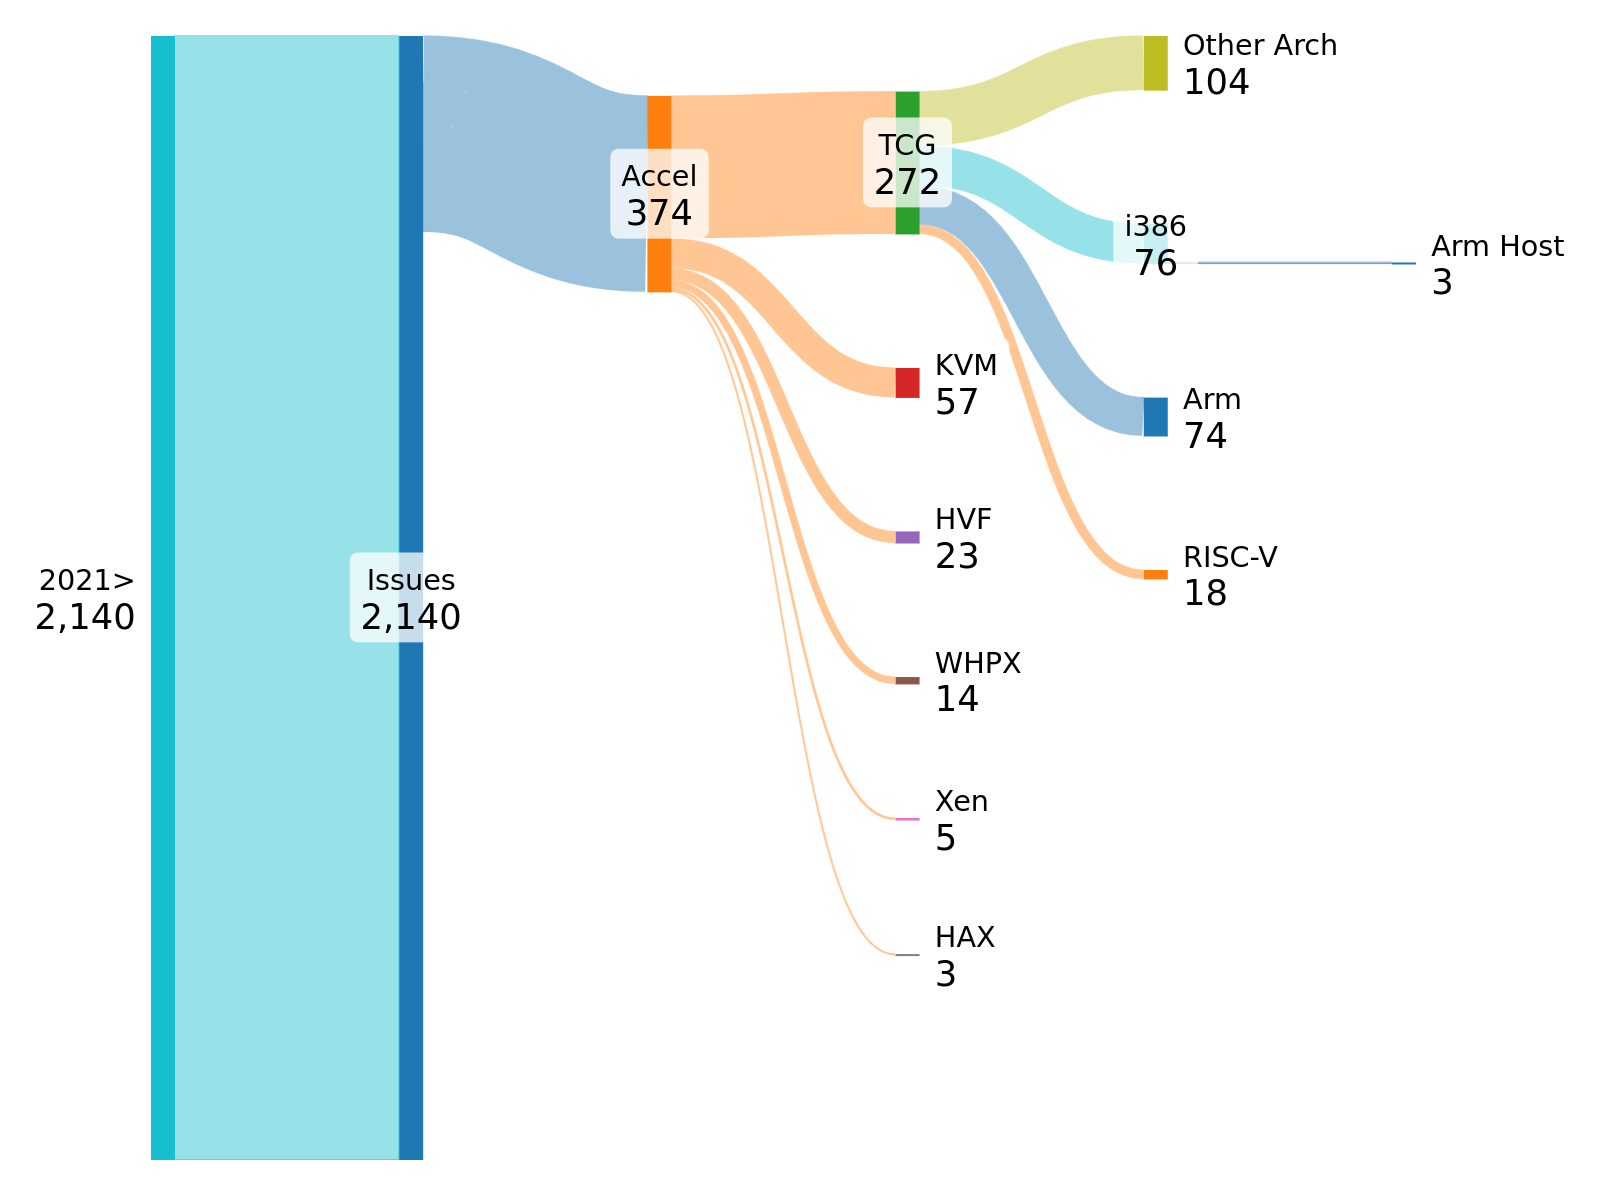
\includegraphics[width=0.8\linewidth]{figures/issues3}
    \caption[QEMU bug distribution]{Sankey diagram showing the distribution of relevant issues}
    \label{fig:issues}
\end{figure}

\section{Distribution of Bugs in \ac{QEMU}}
As is visible in figure \ref{fig:issues} \ac{QEMU} has more than 2000 bugs.
The current version of \ac{QEMU} has 2038147 \ac{sloc} split between different programming and scripting languages according to the line counting program cloc \cite{cloc}.
Drawing from Steve McConnell's research on software metrics \cite{sloc}, we can compare \ac{QEMU}'s bug frequency to that of commercially released products, indicating that \ac{QEMU} has a relatively clean codebase.

Out of all the bugs, 374 are related to accelerators, accounting for about 15\% of the total.
This suggests that the accelerator-related issues are a significant part of the total amount of bugs.
Among these accelerator bugs, the majority, or about 70\%, stem from \ac{TCG}, which is expected given that \ac{TCG} is the primary and most widely used accelerator.
KVM related bugs make up another 15\%, with the remaining 15\% spread across other accelerators.

Regarding \ac{TCG} specific bugs, those involving x86 (i386) and Arm architectures are the most common, each being roughly around 30\% of the total.
This should not come as a surprise since these architectures are being utilized most commonly, leading to extensive usage and testing.

\section{x86 Translation Errors}
In this section, we will go over the bugs encountered when running x86 binaries using the \ac{TCG}.
Most of these bugs are host architecture and operating system independent and tend to arise from incorrect implementation of individual instructions.

We've organized these bugs into six categories based on how they affect the emulation:
\begin{itemize}
    \item Calculation Error: These are mistakes in instructions that either lead to incorrect calculations or issues with flag registers either being incorrectly set or not set at all. However, they don't usually interrupt the flow of the program.
    \item Exceptions: These bugs trigger an exception in \ac{QEMU}, causing the emulation to stop abruptly.
    \item Errors: Similar to exceptions, these issues cause \ac{QEMU} to halt the emulation process.
    \item Segmentation Faults: These occur when the program attempts to access memory areas it doesn't have permission to. While this doesn't happen on actual hardware, it is somehow triggered during the emulation.
    \item Hardware Problems: These bugs impact external hardware, potentially making it unusable or significantly less efficient.
    \item Other Bugs: This category includes bugs that don't fit into the other groups, either because their origin is unclear or because they were introduced in newer versions by mistake.
\end{itemize}

The results of the survey are expressed in the table \ref{tab:tcg_x86}.
In the next sections, we will mainly focus on calculation errors, since this is where the verifier shines the most.
It would be challenging to test the other bugs since they don't necessarily finish their execution normally, therefore leaving the emulator logs incomplete.

\begin{table}[htpb]
    \caption[x86 TCG error distribution]{Distribution of TCG errors for x86.}\label{tab:tcg_x86}
    \centering
    \begin{tabular}{l r r r}
      \toprule
        Type & Number & Closed & Open \\
      \midrule
        Calculation Error & 18 & 12 & 6 \\
        Exceptions & 6 & 4 & 2 \\
        Errors & 3 & 2 & 1 \\
        Segmentation Faults & 14 & 10 & 4 \\
        Hardware Problems & 1 & 0 & 1 \\
        Other & 33 & 26 & 7 \\
      \bottomrule
    \end{tabular}
\end{table}

\subsection{Interpretation and Evaluation of the Bug Survey}

\paragraph{Other:}
As is visible in table \ref{tab:tcg_x86} most errors that originate from x86 emulation belong to this category.
And these errors, make up nearly 45\% of the total amount.
Unfortunately, the bugs that cause these problems are multiple and complex therefore they cannot be easily traced to simple instructions.
Depending on the complexity the verifier can find the bug and the reproducer might be able to reproduce it.
However, it is more than likely that the steps that result in these bugs cannot be simply repeated to pinpoint the actual reason.
Therefore it is quite difficult to reproduce them, making our project a bad match against them.

\paragraph{Hardware Problems:}
There's only a single reported hardware problem, and due to limited information, it's hard to analyze it.
Considering that it is a hardware problem errors of this kind are more likely to be a part of the IO and have nothing to do with emulated instructions.

\paragraph{Segmentation Faults:}
These types of bugs are another frequent issue, accounting for nearly 20\% of all bugs.
A \ac{segfault} happens when a program attempts to access a nonexistent or restricted area.
These accesses can be classified into three categories:
\begin{itemize}
  \item Read
  \item Write
  \item Execute
\end{itemize}
Generally, the best way to solve these bugs is to trace them and find the location where they caused the \ac{segfault}.
In most cases an emulator will keep running and outputting the emulator log until one of the aforementioned events happens.
After the \ac{segfault} happens the the program will be stopped abruptly and the emulator will stop.
This means the emulator log will be stopped before reaching the end.
Even though in the case of a segmentation fault the emulator trace will be cut off, considering that we only need to find the address where this happens along with the used instructions the verifier can be helpful.

Although the verifier can prepare the snapshot and the symbolic expression, the current version only finds errors by comparing states.
This means it will stop before noticing that the emulator log is short.
Theoretically, if the \ac{segfault} is happening because of an instruction the reproducer should be able to reproduce it. 
However, in most cases, this is not possible since the reproducer ignores some details.
A \ac{segfault} happens for multiple reasons, either because the memory location doesn't have the required permissions or because it doesn't exist at all.
However, neither the verifier nor its symbolic log has any knowledge about a memory location's permissions.
Therefore even if we can extract the offending instruction and the used values, without being able to set the memory location's permissions we cannot set an equivalent environment.

In this case, we have two choices.
We can handle it just like other memory access instructions where we allocate space on the data section and then use it for reading or writing.
Or we can keep the original address.
In the first case, we are very likely to not trigger the fault since we use the location that we have declared and made sure it exists.
In the second case, we have no idea whether this original address exists and what its value and permissions are.
Therefore this method would cause undefined behaviour.
Because of these reasons, the reproducer is not a good match for this type of error.
The best we can expect to do is to try the first way and see whether we can trigger the \ac{segfault} consistently.

\paragraph{Errors and Exceptions:}
Errors and exceptions are relatively common in \ac{QEMU}, leading to the program stopping. These issues likely stem from the emulator's internal state, suggesting that alternative debugging methods might be more effective.

\paragraph{Calculation Errors:}
Finally, we have the calculation errors.
They make up slightly less than 25\% of total errors, but they are theoretically the most challenging to detect as they involve instructions behaving slightly differently than expected.
For example, some instructions might set a bit to a wrong value or change another bit that it shouldn't touch.

The main problem with these instructions is that these values are not necessarily used.
This means these programs can go a long way before exhibiting the bug since the difference might have happened multiple instructions ago.
Or maybe the result is close enough to the expected answer and therefore it is not found out.

However, in a good case, this instruction just calculates wrong values, and this discrepancy is detected.
Our verifier and reproducer combination is a good match for these instructions since it uses symbolic execution we can catch every detail and compare it with the emulator log.

\subsection{Detailed Inspection of Bugs on Arm}
In the following subsections, we will go over specific bugs that only appear on Arm devices.
We are inspecting these bugs extra thoroughly because we are interested in seeing whether some bugs appear depending on the host hardware.
Out of 76 bugs that we have seen so far, only 3 of them are Arm specific.
Considering this fact, we can assume that hardware-specific bugs are rather rare.
After taking a closer look at the following subsections, it should be clear that these bugs are not because of the host architecture but because of other reasons.

\subsubsection{Issue \#1659}
The first issue specific to Arm was discovered in an aarch64 system running Darwin.
This bug caused the emulator to freeze and enter a continuous shutdown loop.
It was traced back to the floatx80\_div instruction.
Upon closer examination, it was determined that the problem was due to a miscompilation by Clang.

Therefore, this issue is not directly related to the emulator itself but to the compiler, meaning we can cross this issue from the Arm only list.

\subsubsection{Issue \#2101}
The second issue was identified on a system using Fedora Linux as the host.
This bug manifests itself when executing the ls command within \ac{QEMU}.
It results in incorrect output that omits several directories.
Due to the lack of more information, it is not possible to find the actual cause.

\subsubsection{Issue \#2168}
The final issue also happens in Linux.
This time when running grep on Gentoo Linux inside \ac{QEMU}, a segmentation fault occurs.
Similar to the previous issue, there is limited information available, making it difficult to provide more insights.



